\documentclass[border=4pt]{standalone}
\usepackage{amsmath,amssymb,amsfonts}
\usepackage{xcolor,colortbl,array,booktabs,multirow}
\usepackage{tikz}
\usepackage{pgfplots}
\pgfplotsset{compat=1.16}
\usetikzlibrary{arrows, automata, backgrounds, calendar, chains, decorations,
    matrix, mindmap, patterns, petri, positioning, shadows, shapes.geometric,
    trees, shapes, decorations.pathreplacing, calc, tikzmark, arrows.meta,
    intersections, fit, graphs, quotes, angles, decorations.markings}
\newcommand{\st}{\text{ s.t. }}
\newcommand{\x}{\mathbf{x}}
\renewcommand{\b}{\mathbf{b}}
\renewcommand{\c}{\mathbf{c}}
\newcommand{\A}{\mathbf{A}}
\newcommand{\y}{\mathbf{y}}
\newcommand{\z}{\mathbf{z}}
\newcommand{\R}{\mathbb{R}}
\newcommand{\RR}{\mathbb{R}}
\newcommand{\Z}{\mathbb{Z}}
\newcommand{\ZZ}{\mathbb{Z}}
\newcommand{\npcomplete}{NP-complete}
\providecommand{\true}{\text{TRUE}}
\providecommand{\false}{\text{FALSE}}
\tikzset{vertex/.style={circle,fill=black!25,minimum size=20pt,inner sep=0pt},
    edge/.style={draw,thick,-},weight/.style={font=\small},
    selected vertex/.style={vertex, fill=red!24},
    selected edge/.style={draw,line width=2pt,-,red!50},
    ignored edge/.style={draw,line width=2pt,-,black!20}}
\newcommand{\vect}{\vec}
\providecommand{\ds}{\displaystyle}
\providecommand{\longvect}{\overrightarrow}
\usepackage[normalem]{ulem}
\definecolor{ocre}{RGB}{243,102,25}
\providecommand{\leftB}{\left[}
\providecommand{\rightB}{\right]}
\tikzset{directed/.style={postaction={decorate,decoration={markings,mark=at position .65 with {\arrow{>}}}}},
    directed1/.style={postaction={decorate,decoration={markings,mark=at position .65 with {\arrow{>}}}}}}
\begin{document}
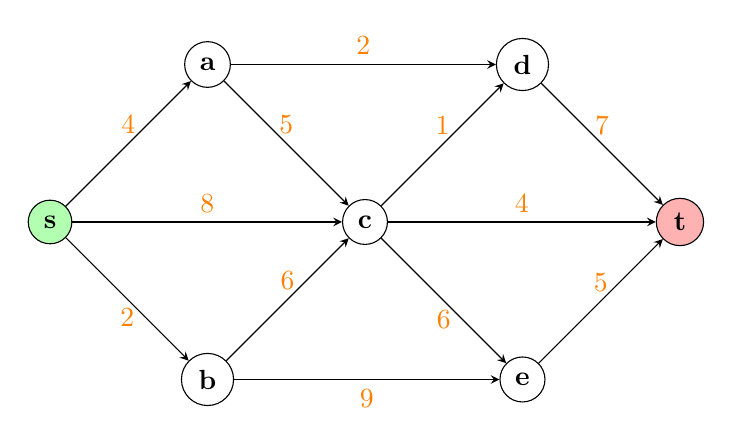
\begin{tikzpicture}[>=stealth, node distance=2cm]

    % Nodes with specific styles
    \node[fill=green,
         fill opacity = 0.3, draw, circle,  text opacity=1] (s) at (0,2) {\textbf{s}};
    \node[draw, circle] (a) at (2,4) {\textbf{a}};
    \node[draw, circle] (b) at (2,0) {\textbf{b}};
    \node[draw, circle] (c) at (4,2) {\textbf{c}};
    \node[draw, circle] (d) at (6,4) {\textbf{d}};
    \node[draw, circle] (e) at (6,0) {\textbf{e}};
    \node[fill=red,
         fill opacity = 0.3, draw, circle,  text opacity=1] (t) at (8,2) {\textbf{t}};

    % Edges with costs (orange, upright)
    \draw[->] (s) -- (a) node[midway, above, text=orange] {4};
    \draw[->] (s) -- (c) node[midway, above, text=orange] {8};
    \draw[->] (s) -- (b) node[midway, below, text=orange] {2};
    \draw[->] (a) -- (c) node[midway, above, text=orange] {5};
    \draw[->] (a) -- (d) node[midway, above, text=orange] {2};
    \draw[->] (c) -- (d) node[midway, above, text=orange] {1};
    \draw[->] (c) -- (t) node[midway, above, text=orange] {4};
    \draw[->] (c) -- (e) node[midway, below, text=orange] {6};
    \draw[->] (b) -- (c) node[midway, above, text=orange] {6};
    \draw[->] (b) -- (e) node[midway, below, text=orange] {9};
    \draw[->] (d) -- (t) node[midway, above, text=orange] {7};
    \draw[->] (e) -- (t) node[midway, above, text=orange] {5};

\end{tikzpicture}
\end{document}
